%!TeX root=../carlo_master.tex
\chapter{Multiclass classification ($K > 2$)}\label{sec:multiclass}

This chapter extends the framework from binary ($K=2$) to the multiclass setting ($K > 2$). The binary case reduces to a scalar threshold on $[0, 1]$; the multiclass problem requires partitioning the probability simplex $\Delta^{K-1}$ into $K$ decision regions with no natural scalar parameterization. We recast the decision stage as a search for a partition of $\Delta^{K-1}$ and show that the standard cost-sensitive rule imposes rigid constraints on the boundary geometry, constraints that can be suboptimal under realistic miscalibration of the estimator.

\section{Geometric analysis of multiclass decision boundaries}\label{sec:geometry}

The decision stage operates on the standard $(K-1)$-simplex
\begin{equation}
    \Delta^{K-1} = \left\{ \mathbf{p} \in \mathbb{R}^K \mid p_i \geq 0 \,\,\, \forall\, i, \, \|\mathbf{p}\|_1 = 1 \right\},
\end{equation}
embedded in $\mathbb{R}^K$. With label space $\mathcal{Y} = \{0, 1, \ldots, K-1\}$, the inference stage produces an estimator $\hat{\mathbf{p}}: \mathcal{X} \to \Delta^{K-1}$, and a decision rule is a measurable map $\delta: \Delta^{K-1} \to \mathcal{Y}$ that induces $K$ disjoint decision regions $\mathcal{P}_i^\delta = \delta^{-1}(\{i\})$ partitioning the simplex. We drop the superscript and write $\mathcal{P}_i$ when the decision rule is unambiguous from context, and use $\mathcal{P}_i^*$ for the closed Bayes Optimal decision regions of Chapter~\ref{sec:theory}, which differ from the assigned regions $\mathcal{P}_i^{\delta^*}$ only on ties.

\section{Bayes optimal polyhedral partitions}

Consider a cost matrix $\mathbf{C} \in \mathbb{R}_{\ge 0}^{K \times K}$. We denote the $i$-th column of $\mathbf{C}$ as the risk vector $\mathbf{c}_i \in \mathbb{R}^K$, the costs of predicting class $i$ across all possible truth labels. Following the convention announced in Section~\ref{sec:theory}, the entry $C_{ij}$ represents the cost incurred by predicting class $j$ when the true class is $i$. The conditional risk of taking action $i$ given a class probability vector $\mathbf{p}$ is the linear functional,
\begin{equation}
    \mathcal{L}_i(\mathbf{p}) = \mathbf{c}_i^\top \mathbf{p} = \sum_{j=0}^{K-1} C_{ji} p_j.
\end{equation}
The functional $\mathcal{L}_i$ takes a generic simplex point as argument and coincides with the conditional risk $\mathcal{R}(i \mid x)$ of Section~\ref{sec:theory} when evaluated at $\mathbf{p} = \boldsymbol{\eta}(x)$.

The Bayes Optimal decision rule $\delta^*$ selects the action minimizing this risk
\begin{equation}\label{eq:multiclass_bayes}
    \delta^*(\mathbf{p}) = \underset{i \in \mathcal{Y}}{\mathrm{argmin}} \,\, \mathbf{c}_i^\top \mathbf{p}.
\end{equation}
We assume a lexicographic tie-breaking rule for the $\mathrm{argmin}$ in~\eqref{eq:multiclass_bayes} to ensure $\delta^*$ is a well-defined function.

\subsection{Admissibility of the cost matrix}

For the cost-sensitive multiclass problem to be well-posed, every class must be optimal for at least one probability vector. A class that is dominated everywhere on the simplex is redundant: no decision rule should ever predict it, and removing it leaves an equivalent problem over the remaining $K-1$ classes. We formalize this through a non-degeneracy condition on $\mathbf{C}$ that generalizes the two-class reasonableness conditions of~\cite{elkan2001foundations}; the element-wise multiclass form of this restriction, in the same simplex-partition setting, appears in~\cite{obrien2008costsensitive}.

\begin{definition}[Admissible cost matrix]\label{def:admissibility}
    A cost matrix $\mathbf{C}$ is admissible if every class $i \in \mathcal{Y}$ is the unique risk-minimizer for at least one valid probability distribution. Formally, for every class $i$, there exists a vector $\mathbf{p} \in \Delta^{K-1}$ such that
    \begin{equation}
        \mathbf{c}_i^\top \mathbf{p} < \mathbf{c}_k^\top \mathbf{p}, \quad \forall k \neq i.
    \end{equation}
    Geometrically, this implies that the decision region $\mathcal{P}_i^*$ for every class has a non-empty interior within the probability simplex.
\end{definition}

\begin{example}[Inadmissible cost matrix]\label{ex:inadmissible}
    Consider a 3-class problem with $\mathcal{Y}=\{0, 1, 2\}$ and cost matrix
    \begin{equation}
        \mathbf{C} = \begin{bmatrix}
            0 & 6 & 10 \\
            4 & 6 & 4 \\
            10 & 6 & 0
        \end{bmatrix}.
    \end{equation}
    Class~1 is the unique risk-minimizer at no $\mathbf{p} \in \Delta^{K-1}$, so $\mathcal{P}_1^* = \emptyset$ and $\mathbf{C}$ is inadmissible. Appendix~\ref{app:supplementary_proofs} gives the verification, including that Class~1 has strictly lower cost than Class~0 in row~2 and than Class~2 in row~0, so no single alternative is element-wise cheaper across every true label and the inadmissibility cannot be read off the entries of $\mathbf{C}$ alone.
\end{example}

The applied cost-sensitive literature commonly works instead with a condition stated directly on the entries of $\mathbf{C}$.

\begin{definition}[Element-wise reasonable cost matrix]\label{def:elementwise}
    A cost matrix $\mathbf{C}$ is element-wise reasonable if, for every true class $j$, a correct prediction costs strictly less than any misprediction,
    \begin{equation}
        C_{jj} < C_{ji}, \quad \forall\, i \neq j.
    \end{equation}
    This is the multiclass form adopted by~\citet{obrien2008costsensitive}; at $K = 2$ it reduces to the reasonableness conditions $C_{00} < C_{01}$ and $C_{11} < C_{10}$ of~\citet{elkan2001foundations}.
\end{definition}

Element-wise reasonableness implies admissibility, but not conversely: a class can have a non-empty decision region without being optimal at any vertex, as the next example shows.

\begin{example}[Admissible matrix violating the element-wise condition]\label{ex:hedge}
    Consider again $\mathcal{Y}=\{0, 1, 2\}$ with
    \begin{equation}
        \mathbf{C} = \begin{bmatrix}
            0 & 10 & 2 \\
            10 & 0 & 2 \\
            3 & 3 & 5
        \end{bmatrix}.
    \end{equation}
    This matrix is admissible but not element-wise reasonable (Definition~\ref{def:elementwise}): class~$2$ is a low-stakes hedge whose correct-prediction cost is not the smallest in its row, so it is risk-optimal at no vertex of $\Delta^{K-1}$, although it is the unique risk-minimizer at the boundary point $(1/2, 1/2, 0)$. Hedge and abstention cost structures populate exactly this gap between the element-wise condition and admissibility; Appendix~\ref{app:supplementary_proofs} gives the verification.
\end{example}

Proposition~\ref{prop:elementwise_admissible} states this relationship in general.

\begin{proposition}[Element-wise reasonableness is strictly stronger than admissibility]\label{prop:elementwise_admissible}
    Let $\mathbf{C} \in \mathbb{R}_{\ge 0}^{K \times K}$.
    \begin{enumerate}
        \item Every element-wise reasonable cost matrix (Definition~\ref{def:elementwise}) is admissible (Definition~\ref{def:admissibility}).
        \item The inclusion is strict for every $K \ge 2$. At $K = 2$ the only admissible matrices outside the element-wise class are obtained by relabeling the two actions; a class that is risk-optimal somewhere in $\Delta^{K-1}$ but at no vertex can occur only for $K \ge 3$, as Example~\ref{ex:hedge} exhibits.
    \end{enumerate}
\end{proposition}

We defer the proof, together with the vertex computations behind Examples~\ref{ex:inadmissible} and~\ref{ex:hedge}, to Appendix~\ref{app:supplementary_proofs}.

Our theoretical results are stated under admissibility, the weaker of the two conditions. This is a scope choice, not a claim that element-wise reasonableness is deficient: the proofs that invoke admissibility use it only through the non-emptiness of each Bayes region, so the weaker hypothesis is all they require. Example~\ref{ex:inadmissible} shows a matrix that is not even admissible, and Example~\ref{ex:hedge} one that is admissible but not element-wise reasonable. The empirical campaign (Chapters~\ref{sec:binary_experiments} and~\ref{sec:multiclass_experiments}) uses element-wise reasonable cost matrices, following the applied cost-sensitive literature; by Proposition~\ref{prop:elementwise_admissible}(1) these are admissible, so the theory transfers to the experimental setting unchanged.

\subsection{Cost-determined geometry of the Bayes partition}

Under admissibility, the minimization in Eq.~(\ref{eq:multiclass_bayes}) induces a polyhedral partition of the simplex whose boundary normals are determined entirely by the cost matrix.

\begin{theorem}[Rigid polyhedral partition]\label{thm:rigid_partition}
    Given an admissible cost matrix $\mathbf{C}$, the closed Bayes Optimal decision regions are convex polyhedra that cover $\Delta^{K-1}$. They can overlap where conditional risks tie; assigning each tie to its smallest-index minimizer gives a partition. The boundary separating any two adjacent regions $\mathcal{P}_i$ and $\mathcal{P}_j$ lies on the hyperplane $\mathcal{B}_{ij}$ defined by
    \begin{equation}
        \mathcal{B}_{ij} = \{ \mathbf{p} \in \mathbb{R}^K \mid (\mathbf{c}_i - \mathbf{c}_j)^\top \mathbf{p} = 0 \}.
    \end{equation}
    The normal vector to the separating boundary is fixed as $\mathbf{n}_{ij} = \mathbf{c}_i - \mathbf{c}_j$.
\end{theorem}

\begin{proof}
    A point $\mathbf{p}$ belongs to the closed region $\mathcal{P}_i$ if the risk of action $i$ is lower than or equal to the risk of any other action $k$. This can be expressed as an intersection of linear inequalities,
    \begin{equation}\label{eq:region_def}
        \mathcal{P}_i = \bigcap_{k \neq i} \left\{ \mathbf{p} \in \Delta^{K-1} \mid \mathbf{c}_i^\top \mathbf{p} \le \mathbf{c}_k^\top \mathbf{p} \right\}
              = \bigcap_{k \neq i} \left\{ \mathbf{p} \in \Delta^{K-1} \mid (\mathbf{c}_i - \mathbf{c}_k)^\top \mathbf{p} \le 0 \right\}.
    \end{equation}
    Each term $(\mathbf{c}_i - \mathbf{c}_k)^\top \mathbf{p} \le 0$ defines a closed half-space in $\mathbb{R}^K$. Since the simplex $\Delta^{K-1}$ is a convex polytope, and the intersection of convex sets is convex, the resulting region $\mathcal{P}_i$ is a convex polytope. The boundary between regions $i$ and $j$ is the set where risks are equal, $\mathbf{c}_i^\top \mathbf{p} = \mathbf{c}_j^\top \mathbf{p}$, which defines the hyperplane with normal vector $\mathbf{c}_i - \mathbf{c}_j$.
\end{proof}

By Theorem~\ref{thm:rigid_partition} the boundary orientation $\mathbf{n}_{ij} = \mathbf{c}_i - \mathbf{c}_j$ is fixed by $\mathbf{C}$ alone, while the estimation error $\boldsymbol{\epsilon}(x) = \hat{\mathbf{p}}(x) - \boldsymbol{\eta}(x)$ is governed by the estimator's inductive bias and is unconstrained relative to that orientation. The plug-in rule decides the $i$ versus $j$ boundary on $\mathbf{n}_{ij}^\top \hat{\mathbf{p}}(x)$ rather than $\mathbf{n}_{ij}^\top \boldsymbol{\eta}(x)$, so it inverts the Bayes decision at $x$ exactly when the two have opposite signs, that is when $|\mathbf{n}_{ij}^\top \boldsymbol{\epsilon}(x)| > |\mathbf{n}_{ij}^\top \boldsymbol{\eta}(x)|$ with $\boldsymbol{\epsilon}(x)$ opposing $\boldsymbol{\eta}(x)$ along $\mathbf{n}_{ij}$. Since the orientation cannot adapt to this error, Chapter~\ref{sec:partition_optimization} fits the boundary to validation data instead of deriving it from $\mathbf{C}$.

\begin{figure}[H]
    \centering
    \resizebox{0.8\textwidth}{!}{\documentclass[tikz, border=10pt]{standalone}
\usepackage{tikz}
\usepackage{amsmath}
\usetikzlibrary{shapes, calc, backgrounds, arrows.meta}

\begin{document}
\begin{tikzpicture}[font=\sffamily]

    \begin{scope}[xshift=0.0cm, scale=0.65]
    \coordinate (Top) at (0.000, 5.000);
    \coordinate (Right) at (4.330, -2.500);
    \coordinate (Left) at (-4.330, -2.500);

    \coordinate (Int) at (0.000, 0.000);

    \fill[green!15] (0.000, 5.000) -- (2.165, 1.250) -- (0.000, 0.000) -- (-2.165, 1.250) -- cycle;
    \fill[blue!15] (4.330, -2.500) -- (0.000, -2.500) -- (0.000, 0.000) -- (2.165, 1.250) -- cycle;
    \fill[red!15] (-4.330, -2.500) -- (-2.165, 1.250) -- (0.000, 0.000) -- (0.000, -2.500) -- cycle;

    \draw[thick, black!50] (Int) -- (2.165, 1.250);
    \draw[thick, black!50] (Int) -- (-2.165, 1.250);
    \draw[thick, black!50] (Int) -- (0.000, -2.500);

    \draw[thick] (Top) -- (Right) -- (Left) -- cycle;

    \node[green!50!black, font=\small\bfseries] at (0.000, 2.500) {$\mathcal{P}_0$};
    \node[blue!70!black, font=\small\bfseries] at (2.000, -1.000) {$\mathcal{P}_1$};
    \node[red!70!black, font=\small\bfseries] at (-2.000, -1.000) {$\mathcal{P}_2$};

    \node[above, font=\small] at (Top) {$\mathbf{e}_0$};
    \node[right, font=\small] at (Right) {$\mathbf{e}_1$};
    \node[left, font=\small] at (Left) {$\mathbf{e}_2$};
    \node[font=\small\bfseries, anchor=north, align=center] at (0, -2.750) {(a) $C_{ij} = 1 \;\forall\, i \neq j$};
    \end{scope}

    \begin{scope}[xshift=8.0cm, scale=0.65]
    \coordinate (Top) at (0.000, 5.000);
    \coordinate (Right) at (4.330, -2.500);
    \coordinate (Left) at (-4.330, -2.500);

    \coordinate (Int) at (0.962, 1.667);

    \fill[green!15] (0.000, 5.000) -- (2.165, 1.250) -- (0.962, 1.667) -- (-0.722, 3.750) -- cycle;
    \fill[blue!15] (4.330, -2.500) -- (2.165, -2.500) -- (0.962, 1.667) -- (2.165, 1.250) -- cycle;
    \fill[red!15] (-4.330, -2.500) -- (-0.722, 3.750) -- (0.962, 1.667) -- (2.165, -2.500) -- cycle;

    \draw[thick, black!50] (Int) -- (2.165, 1.250);
    \draw[thick, black!50] (Int) -- (-0.722, 3.750);
    \draw[thick, black!50] (Int) -- (2.165, -2.500);

    \draw[dashed, gray!50, thin] (Left) -- (2.165, 1.250);
    \draw[dashed, gray!50, thin] (Right) -- (-2.165, 1.250);
    \draw[dashed, gray!50, thin] (Top) -- (0.000, -2.500);

    \draw[thick] (Top) -- (Right) -- (Left) -- cycle;

    % Normal vector annotations
    \coordinate (NormStart) at (1.564, 1.458);
    \draw[->, >=Stealth, thick, black!70] (NormStart) -- ++(0.524, 1.512)
        node[above left, font=\footnotesize] {$\mathbf{n}_{01}$};
    \coordinate (NormStart) at (0.120, 2.708);
    \draw[->, >=Stealth, thick, black!70] (NormStart) -- ++(-1.244, -1.006)
        node[below right, font=\footnotesize] {$\mathbf{n}_{20}$};
    \coordinate (NormStart) at (1.564, -0.417);
    \draw[->, >=Stealth, thick, black!70] (NormStart) -- ++(1.537, 0.444)
        node[below right, font=\footnotesize] {$\mathbf{n}_{12}$};

    \node[green!50!black, font=\small\bfseries] at (0.300, 3.500) {$\mathcal{P}_0$};
    \node[blue!70!black, font=\small\bfseries] at (2.800, -1.000) {$\mathcal{P}_1$};
    \node[red!70!black, font=\small\bfseries] at (-1.800, -0.500) {$\mathcal{P}_2$};

    \node[above, font=\small] at (Top) {$\mathbf{e}_0$};
    \node[right, font=\small] at (Right) {$\mathbf{e}_1$};
    \node[left, font=\small] at (Left) {$\mathbf{e}_2$};
    \node[font=\small\bfseries, anchor=north, align=center] at (0, -2.750) {(b) $C_{20}{=}5,\; C_{21}{=}3$};
    \end{scope}

\end{tikzpicture}
\end{document}
}
    \caption{Bayes-optimal decision regions on the 3-class probability simplex. \textbf{(a)}~Under symmetric 0/1 loss, boundaries are the medians meeting at the barycenter $(1/3, 1/3, 1/3)$, yielding equal-sized regions. \textbf{(b)}~Under asymmetric costs with $C_{ii}=0$, $C_{20}=5$, $C_{21}=3$, and all other off-diagonal entries equal to~1, the boundaries rotate and the intersection shifts to $(5/9, 1/3, 1/9)$, expanding $\mathcal{P}_2$ at the expense of $\mathcal{P}_0$ and $\mathcal{P}_1$. The normal vectors $\mathbf{n}_{ij} = \mathbf{c}_i - \mathbf{c}_j$ are determined entirely by the cost matrix (Theorem~\ref{thm:rigid_partition}).}\label{fig:simplex_cost_partition}
\end{figure}

The same partition admits a three-dimensional reading. Graphing each conditional-risk functional $\mathcal{L}_i(\mathbf{p}) = \mathbf{c}_i^\top \mathbf{p}$ as a plane over $\Delta^{K-1}$, the Bayes rule selects the lowest plane at each $\mathbf{p}$, and the orthogonal projection of this lower envelope onto the simplex base reproduces the 2D partition; Figure~\ref{fig:simplex_cost_partition_3d} renders both cost matrices in this view.

\begin{figure}[H]
    \centering
    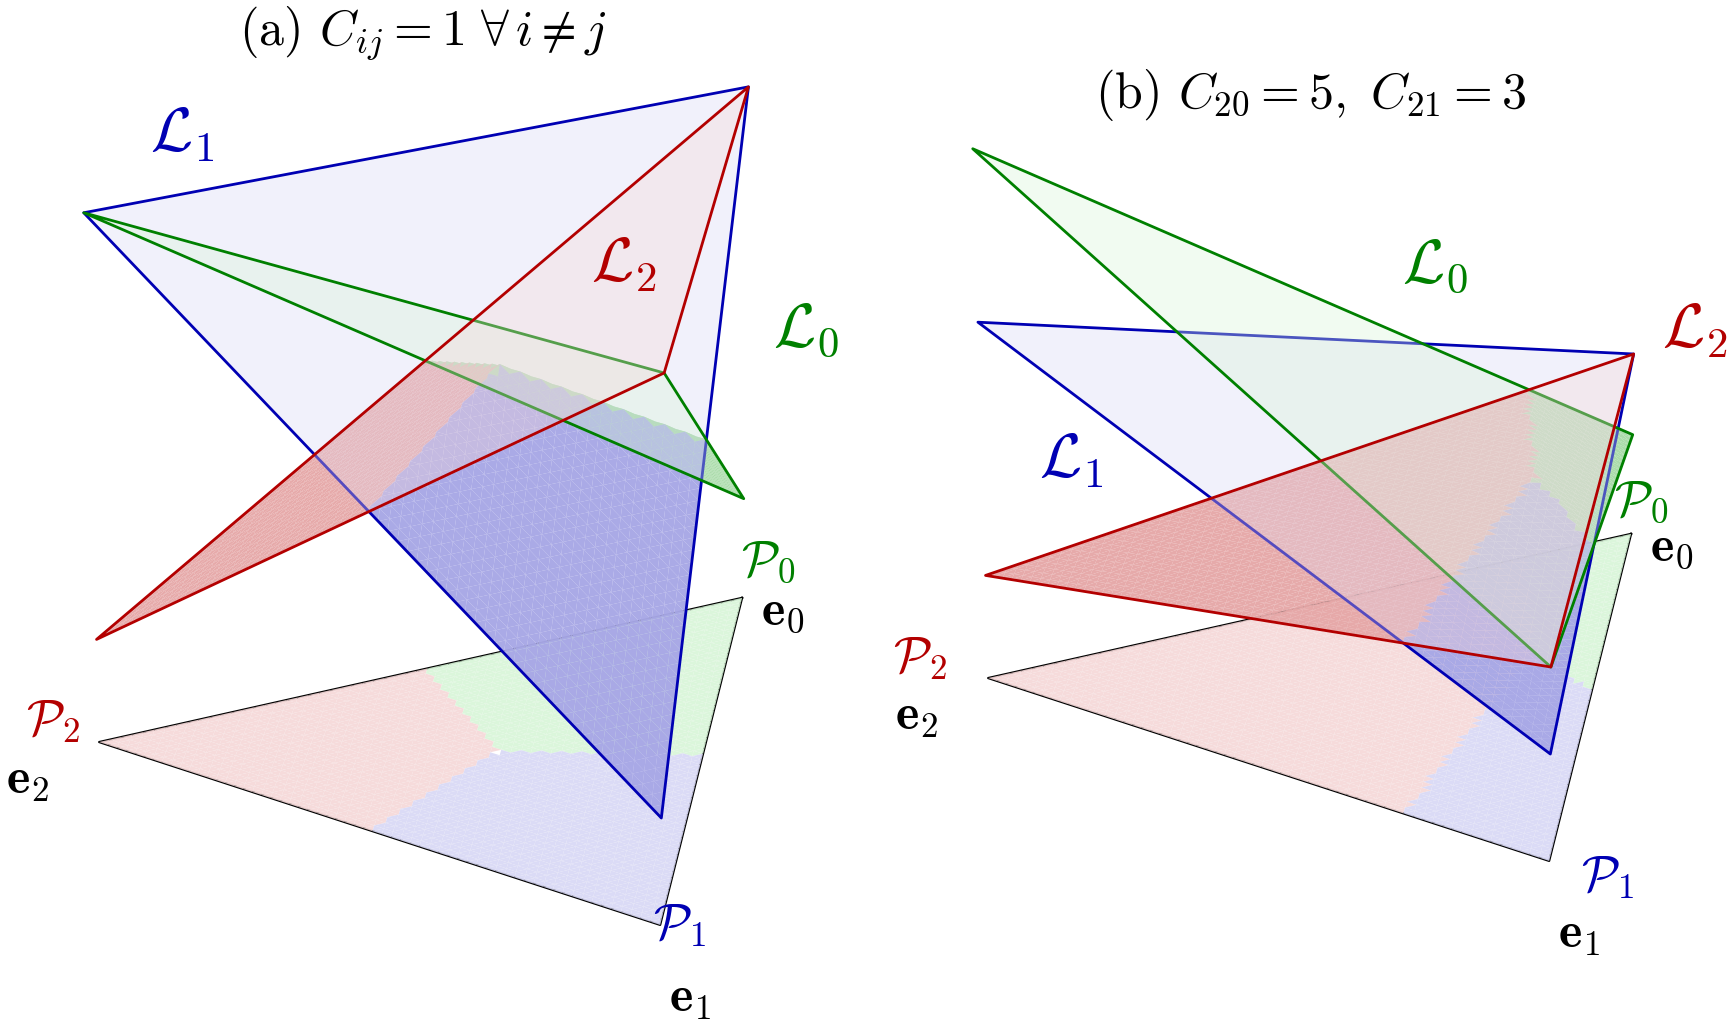
\includegraphics[width=0.72\textwidth]{figures/simplex_cost_partition_3d.png}
    \caption{Risk planes and lower envelope on the 3-class probability simplex, for the same cost matrices as Figure~\ref{fig:simplex_cost_partition}. Each semi-transparent plane graphs a conditional-risk functional $\mathcal{L}_i(\mathbf{p}) = \mathbf{c}_i^\top \mathbf{p}$ over $\Delta^2$; the opaque facets are the lower envelope $\min_i \mathcal{L}_i$, one facet per region $\mathcal{P}_i^*$ on which action $i$ is risk-minimal. Projecting the envelope vertically onto the simplex base recovers the 2D partition of Figure~\ref{fig:simplex_cost_partition}. \textbf{(a)}~Symmetric 0/1 loss yields three congruent planes meeting at the barycenter and three equal-area envelope facets. \textbf{(b)}~Under asymmetric costs $C_{20}=5,\ C_{21}=3$, plane $\mathcal{L}_2$ has steeper slopes against $\mathbf{e}_0$ and $\mathbf{e}_1$, and $\mathcal{P}_2^*$ expands at the expense of $\mathcal{P}_0^*$ and $\mathcal{P}_1^*$.}\label{fig:simplex_cost_partition_3d}
\end{figure}

\section{Limitations of the plug-in rule in the multiclass setting}\label{sec:analytical_fragility}

As in the binary case, the standard approach applies the Bayes Optimal projection (Eq.~\ref{eq:multiclass_bayes}) directly to the estimated probabilities,
\begin{equation}
    \hat{h}(x) = \underset{i \in \mathcal{Y}}{\mathrm{argmin}} \,\, \mathbf{c}_i^\top \hat{\mathbf{p}}(x).
\end{equation}
This rule attains the Bayes risk whenever, for almost every $x$, its selected action minimizes the conditional risk at the true posterior; exact posterior recovery, $\hat{\mathbf{p}}(x) = \boldsymbol{\eta}(x)$ almost everywhere, is sufficient for this but not necessary. In practice, systematic estimation errors shift the distribution of estimates within the simplex, creating a geometric mismatch between the theoretical boundaries from $\mathbf{C}$ and the effective support of the estimator.

\subsection{Systematic estimation error in the probability simplex}

Let $\Psi: \Delta^{K-1} \to \Delta^{K-1}$ denote the systematic distortion induced by the estimator, so that
$\hat{\mathbf{p}}(x) \approx \Psi(\boldsymbol{\eta}(x))$. Two common distortion regimes are especially relevant.

\paragraph{Oversmoothing.}
Strong regularization shrinks estimated probabilities toward the barycenter
$\mathbf{u} = (1/K,\ldots,1/K)^\top$. As a result, estimates may never reach the parts of the simplex where a high-penalty or minority class is Bayes-optimal. The plug-in classifier can then fail to predict that class at all, even when the estimator preserves the correct ranking among class probabilities.

\paragraph{Undersmoothing.}
At the opposite extreme, overconfident estimators push $\hat{\mathbf{p}}(x)$ toward the vertices of the simplex. If $\hat{\mathbf{p}}(x) \approx \mathbf{e}_i$, then the risk of predicting class $k$ is approximately $C_{ik}$, and the plug-in rule chooses the cheapest action in row $i$ of the cost matrix. Under element-wise reasonableness, this is simply class $i$, since $C_{ii} < C_{ik}$ for all $k \neq i$. Thus the decision reduces to the cost-blind argmax rule, and the magnitudes of the off-diagonal costs have little practical effect.

Figure~\ref{fig:simplex_distortions} illustrates these two distortions on the 3-class simplex.

\begin{figure}[H]
    \centering
    \resizebox{\textwidth}{!}{\documentclass[tikz, border=10pt]{standalone}
\usepackage{tikz}
\usepackage{amsmath}
\usetikzlibrary{calc, arrows.meta}

\begin{document}
\begin{tikzpicture}[font=\sffamily]

    % ===== LEFT PANEL: Oversmoothing =====
    \begin{scope}[scale=0.65]
        % Vertices
        \coordinate (T) at (0, 5);
        \coordinate (R) at (4.33, -2.5);
        \coordinate (L) at (-4.33, -2.5);

        % Centroid and edge midpoints
        \coordinate (G) at (0, 0);
        \coordinate (MidTR) at (2.165, 1.25);
        \coordinate (MidTL) at (-2.165, 1.25);
        \coordinate (MidRL) at (0, -2.5);

        % Light region fills (same as 0/1 loss partition)
        \fill[green!8] (T) -- (MidTR) -- (G) -- (MidTL) -- cycle;
        \fill[blue!8] (R) -- (MidRL) -- (G) -- (MidTR) -- cycle;
        \fill[red!8] (L) -- (MidTL) -- (G) -- (MidRL) -- cycle;

        % Triangle frame
        \draw[thick] (T) -- (R) -- (L) -- cycle;

        % Contraction arrows (showing direction of distortion toward centroid)
        \draw[->, >=Stealth, gray!60, thick, shorten >=6pt] (0, 3.5) -- (0, 1.2);
        \draw[->, >=Stealth, gray!60, thick, shorten >=6pt] (2.8, -1.3) -- (0.9, -0.2);
        \draw[->, >=Stealth, gray!60, thick, shorten >=6pt] (-2.8, -1.3) -- (-0.5, 0.5);

        % Estimated points colored by TRUE class, all clustered near centroid
        % Class 0 (green) — estimates still in R_0
        \node[circle, fill=green!60!black, inner sep=1.3pt] at (0.2, 1.3) {};
        \node[circle, fill=green!60!black, inner sep=1.3pt] at (-0.4, 1.0) {};
        \node[circle, fill=green!60!black, inner sep=1.3pt] at (0.5, 0.8) {};

        % Class 1 (blue) — estimates still in R_1
        \node[circle, fill=blue!80, inner sep=1.3pt] at (0.9, 0.1) {};
        \node[circle, fill=blue!80, inner sep=1.3pt] at (0.7, -0.3) {};
        \node[circle, fill=blue!80, inner sep=1.3pt] at (1.1, -0.1) {};

        % Class 2 (red) — estimates in R_0, NOT in R_2 (misclassified)
        \node[circle, fill=red!80, inner sep=1.3pt] at (-0.4, 0.5) {};
        \node[circle, fill=red!80, inner sep=1.3pt] at (-0.2, 0.4) {};
        \node[circle, fill=red!80, inner sep=1.3pt] at (-0.7, 0.6) {};

        % Vertex labels
        \node[above, font=\small] at (T) {$\mathbf{e}_0$};
        \node[right, font=\small] at (R) {$\mathbf{e}_1$};
        \node[left, font=\small] at (L) {$\mathbf{e}_2$};

        % Panel label
        \node[font=\small\bfseries, anchor=north west] at (-4.33, 5.5) {(a)};
    \end{scope}

    % ===== RIGHT PANEL: Undersmoothing =====
    \begin{scope}[xshift=8cm, scale=0.65]
        % Vertices
        \coordinate (T) at (0, 5);
        \coordinate (R) at (4.33, -2.5);
        \coordinate (L) at (-4.33, -2.5);

        % Centroid and edge midpoints
        \coordinate (G) at (0, 0);
        \coordinate (MidTR) at (2.165, 1.25);
        \coordinate (MidTL) at (-2.165, 1.25);
        \coordinate (MidRL) at (0, -2.5);

        % Light region fills
        \fill[green!8] (T) -- (MidTR) -- (G) -- (MidTL) -- cycle;
        \fill[blue!8] (R) -- (MidRL) -- (G) -- (MidTR) -- cycle;
        \fill[red!8] (L) -- (MidTL) -- (G) -- (MidRL) -- cycle;

        % Triangle frame
        \draw[thick] (T) -- (R) -- (L) -- cycle;

        % Expansion arrows (showing direction of distortion toward vertices)
        \draw[->, >=Stealth, gray!60, thick, shorten >=6pt] (0, 2.0) -- (0, 3.8);
        \draw[->, >=Stealth, gray!60, thick, shorten >=6pt] (1.2, -0.5) -- (3.2, -1.8);
        \draw[->, >=Stealth, gray!60, thick, shorten >=6pt] (-1.2, -0.5) -- (-3.2, -1.8);

        % Data points clustered near vertices (overconfident)
        % Class 0 near Top
        \node[circle, fill=green!60!black, inner sep=1.3pt] at (-0.1, 4.3) {};
        \node[circle, fill=green!60!black, inner sep=1.3pt] at (0.3, 4.0) {};
        \node[circle, fill=green!60!black, inner sep=1.3pt] at (-0.25, 3.8) {};

        % Class 1 near Right
        \node[circle, fill=blue!80, inner sep=1.3pt] at (3.8, -2.1) {};
        \node[circle, fill=blue!80, inner sep=1.3pt] at (3.5, -1.8) {};
        \node[circle, fill=blue!80, inner sep=1.3pt] at (3.6, -2.4) {};

        % Class 2 near Left
        \node[circle, fill=red!80, inner sep=1.3pt] at (-3.8, -2.1) {};
        \node[circle, fill=red!80, inner sep=1.3pt] at (-3.5, -1.8) {};
        \node[circle, fill=red!80, inner sep=1.3pt] at (-3.6, -2.4) {};

        % Annotation
        \node[black!70, font=\footnotesize, align=center] at (0, -0.2)
            {$\hat{\mathbf{p}} \approx \mathbf{e}_k$};

        % Vertex labels
        \node[above, font=\small] at (T) {$\mathbf{e}_0$};
        \node[right, font=\small] at (R) {$\mathbf{e}_1$};
        \node[left, font=\small] at (L) {$\mathbf{e}_2$};

        % Panel label
        \node[font=\small\bfseries, anchor=north west] at (-4.33, 5.5) {(b)};
    \end{scope}

\end{tikzpicture}
\end{document}
}
    \caption{Effects of estimation error on the 3-class simplex. \textbf{(a)}~Probability contraction (oversmoothing) shrinks the estimator's image $\mathrm{Im}(\Psi)$ into a sub-region $\mathcal{S}$ near the barycenter. If $\mathcal{S}$ does not intersect $\mathcal{P}_2^*$, the classifier has zero recall for class~2 even though the decision boundary is correct. \textbf{(b)}~Overconfidence (undersmoothing) pushes estimates toward vertices ($\hat{\mathbf{p}} \approx \mathbf{e}_k$), making all points fall deep inside their respective argmax regions. The cost structure becomes irrelevant since $\mathrm{argmin}_{k \in \mathcal{Y}} \mathbf{c}_k^\top \hat{\mathbf{p}}$ reduces to $\mathrm{argmax}_{k \in \mathcal{Y}} \hat{p}_k$.}\label{fig:simplex_distortions}
\end{figure}

\subsection{The inverse-map problem}

Even when $\Psi$ is a bijection on $\Delta^{K-1}$ and the discriminative ranking is preserved, the analytical rule applied in the estimate space is not Bayes-optimal. The analytical boundary lives in the true-probability space, $\mathcal{B}_{ij} = \{\mathbf{p} \in \mathbb{R}^K \mid (\mathbf{c}_i - \mathbf{c}_j)^\top \mathbf{p} = 0\}$, so the corresponding boundary in the estimate space is its pre-image
\begin{equation}
    \tilde{\mathcal{B}}_{ij} = \Psi^{-1}(\mathcal{B}_{ij}) = \{ \mathbf{z} \in \Delta^{K-1} \mid (\mathbf{c}_i - \mathbf{c}_j)^\top \Psi^{-1}(\mathbf{z}) = 0 \}.
\end{equation}
Because $\Psi$ is generically non-linear, $\tilde{\mathcal{B}}_{ij}$ is a curved manifold, not a hyperplane. Applying the analytical rule with the fixed normals $\mathbf{n}_{ij} = \mathbf{c}_i - \mathbf{c}_j$ in estimate space therefore introduces an approximation error that translation alone cannot eliminate. Two corrective routes follow: estimate $\Psi^{-1}$ with a low-parameter family before applying the analytical rule (post-hoc calibration, Section~\ref{sec:multiclass_calibration}), or skip the inverse map entirely and learn a new partition of the estimate simplex directly (Chapter~\ref{sec:partition_optimization}).

\section{Post-hoc calibration in the multiclass setting}\label{sec:multiclass_calibration}

Multiclass perfect calibration requires $\mathbb{P}(Y{=}k \mid \hat{\mathbf{p}}(X) = \mathbf{q}) = q_k$ for all $k$ and almost every $\mathbf{q} \in \Delta^{K-1}$ under the law of $\hat{\mathbf{p}}(X)$, a joint condition over the simplex strictly stronger than the per-class binary condition (Definition~\ref{def:calibration}). The calibrators that extend the binary methods to $K > 2$ trade off in how much of this joint structure they attempt to model.

\paragraph{Temperature scaling.} The most conservative extension \citep{guo2017calibration} applies a single scalar $T > 0$ to the logit vector before the softmax: $g_T(\hat{\mathbf{p}}) = \mathrm{softmax}(\mathbf{z}/T)$ with $z_k = \log \hat{p}_k$. Like its binary analogue, it preserves the ranking of all $K$ classes and has only one degree of freedom, so it is the most data-efficient option but cannot redistribute mass between classes asymmetrically.

\paragraph{Platt scaling.} Extends temperature scaling by a one-vs-rest decomposition: each class $k$ receives its own two-parameter sigmoid calibrator fitted on the binary task ``class $k$ vs.\ rest'', and the $K$ outputs are renormalized to sum to one. The total parameter count is $2K$, so the family can correct class-specific overconfidence but ignores cross-class interactions: the calibrator for class $k$ is blind to the joint shape of the score distribution over the other $K-1$ classes.

\paragraph{Isotonic regression.} Applies the same one-vs-rest decomposition with non-parametric monotone calibrators in place of the sigmoid; its complexity is adaptive in the calibration-set size rather than fixed in $K$, and it inherits the same cross-class blindness.

\paragraph{Dirichlet calibration.} Natively multiclass \citep{kull2019beyond}, this calibrator models exactly those cross-class interactions. The full parameterization
\[
g_{\mathbf{W},\mathbf{b}}(\hat{\mathbf{p}}) = \mathrm{softmax}(\mathbf{W} \log \hat{\mathbf{p}} + \mathbf{b}),
\quad \mathbf{W} \in \mathbb{R}^{K \times K},\; \mathbf{b} \in \mathbb{R}^K
\]
(Eq.~\ref{eq:dirichlet_calibration}) acts as a log-linear transformation on the simplex with $K^2 + K$ free parameters. Setting $\mathbf{W} = (1/T)\,\mathbf{I}$ with $\mathbf{b} = \mathbf{0}$ recovers temperature scaling, and the full $\mathbf{W}$ is the maximally expressive log-linear case; intermediate restrictions on $\mathbf{W}$ correspond to the vector and matrix scaling variants of \citet{guo2017calibration}.

The parametric calibrators can be ordered by flexibility. Temperature scaling uses a single parameter and preserves the class ranking, so it can correct global overconfidence but not class-specific distortions. One-vs-rest Platt scaling introduces $2K$ parameters and can correct per-class miscalibration, but because each class is calibrated against the rest independently, it does not model cross-class interactions. Dirichlet calibration is the most expressive of the three: with $K^2+K$ parameters, it applies a log-linear transformation to the full probability vector and can represent interactions among classes. Isotonic regression occupies a separate position in the comparison, since its non-parametric monotone complexity depends on the calibration-set size rather than on a fixed parameter count in $K$.

Each calibrator can be composed with either the cost-blind argmax rule or the analytical cost-sensitive rule in Eq.~\ref{eq:multiclass_bayes}, yielding a \textit{calibrate-then-decide} strategy. As in the binary case, the argument of Proposition~\ref{prop:calibrate_then_decide} extends: recovering the true posterior vector, $g(\hat{\mathbf{p}}(x)) = \boldsymbol{\eta}(x)$ almost everywhere, makes the analytical rule applied to $g(\hat{\mathbf{p}}(x))$ attain the Bayes risk. Perfect multiclass calibration alone does not imply this posterior-recovery condition. In practice, calibration is only approximate, and the remaining distortion motivates the direct partition-optimization strategies of Chapter~\ref{sec:partition_optimization}.
